\documentclass[11pt]{article}
\usepackage{eacl2017}
\usepackage{times}
\usepackage{url}
\usepackage{latexsym}
\usepackage{graphicx}
\usepackage{multirow}



\newcommand\BibTeX{B{\sc ib}\TeX}

\title{Sanskrit Sandhi Splitting and Merging: Benchmark Datasets and Evaluation}

\author{Neelamadhav Gantayat\\
	IBM Research \\
	Bangalore, India \\
	{\tt neelamadhav@in.ibm.com} \\\And
	Shubham Bhardwaj \\
	IIT Delhi \\
	New Delhi, India \\
	{\tt ee1120480@ee.iitd.ac.in} \\\And
	Dr. Rahul Garg \\
	 IIT Delhi \\
	  New Delhi, India \\
	  {\tt rahulgarg@cse.iitd.ac.in} \\\And
	  Dr. Sumeet Agarwal \\
	  IIT Delhi \\
	 New Delhi, India \\
	  {\tt sumeet@ee.iitd.ac.in} \\}

\date{}

\begin{document}
	\maketitle
\begin{abstract}
	Words in Sanskrit language are formed by a process called Sandhi merging, which is a combination of two or more morphemes (component words). The reverse process of getting back the component words from the full words is known as Sandhi splitting. Learning the fundamentals of an old language, such as Sanskrit, will provide insights to the overall community of language modeling. It is believed by many scholars that though \textit{P\={a}\d{n}ini} has written a grammar for Sanskrit words, called \textit{A\d{s}\d{t}\={a}dhy\={a}y\={\i}}. Analyzing and understanding word formation in Sanskrit is conceptually generic providing us with a framework to write grammars for other languages. However, the publicly available dataset such as the University of Hyderabad dataset is very erroneous making it challenging to design and evaluate automated algorithms. The primary contribution of this research work is to create a set of public datasets with manually created ground truth for promoting research in this fundamental problem. Further, we present the results of three publicly available tools for performing Sandhi splitting and Sandhi merging and benchmark their performance. We finally discuss the characteristics of each of the tool and emphasize the need for further research.
\end{abstract}

\section{Introduction}

The basic constituents of a language are its characters which are joined together to form morphemes, which is the meaning fundamental part of a language that cannot further divided. Morphemes are combined together to form words, words are combined to form sentences, and sentences are combined to form large texts. The purpose of a language model is to understand the underlying rules and structure that comprises a language. There are two broad approaches for constructing a language model as follows:
\begin{itemize}
	\item \textbf{Grammar based model:} This approach is generally used to model complex but deterministic grammar based languages. The learning models can be rule based or typically require less training data.
	\item \textbf{Probabilistic based model:} When a deterministic grammar is not available, a probabilistic language model can be learnt using a large corpus of data.
\end{itemize}

\begin{table*}[t]
	\begin{center}
		\begin{tabular}{|p{1.2cm}|l|l|l|}
			\hline 
			\bf Criteria	& \bf Type	& \bf Explanation	& \bf Example \\
			\hline
			
			\multirow{2}{*}{Position} & Internal &  Morphemes combine to form word &\textit{ bho} + \textit{anam}  $\rightarrow$ \textit{bhavanam } \\ \cline{2-4} 
			
			& External & Words combine to form compound words & \textit{tau} + \textit{ekad\={a}} $\rightarrow$ \textit{t\={a}vekad\={a}}  \\ \hline \hline
			
			\multirow{3}{*}{\parbox{1.2cm}{Type of character}} & Vowel &  Both joining letters are vowels  & \textit{ hima} + \textit{ \={a}laya\d{h}} $\rightarrow$ \textit{him\={a}laya\d{h}}  \\ \cline{2-4} 
			
			& Consonant &  One of the two letters is a consonant & \textit{v\d{r}k\d{s}a} + \textit{ch\={a}y\={a} } $\rightarrow$ \textit{v\d{r}k\d{s}acch\={a}y\={a}} 
			\\ \cline{2-4}
			
			& Visarga &  Visarga with a vowel or a consonant &  \textit{ puna\d{h} } + \textit{janma } $\rightarrow$ \textit{punarjanma}    \\ \hline 
			
		\end{tabular}
	\end{center}
	\caption{\label{typestable} Different types of Sandhi classification}
\end{table*}

Sanskrit is one of the oldest languages designed by mankind having its origin in the Indo-Aryan civilization from 200B.C. Sanskrit has a rich tradition of poetry and literature works written, making it an important linguistic study. Being one of the oldest language, word formation in Sanskrit can be defined by set of deterministic rules and follows a defined structure. \textit{A\d{s}\d{t}\={a}dhy\={a}y\={\i}} (meaning a collection of eight books) by \textit{P\={a}\d{n}ini} is the source of Sanskrit's grammar, syntax, and semantics. The importance of \textit{a\d{s}\d{t}\={a}dhy\={a}y\={\i}} is three fold~\cite{bharati2007}. The first one, as is well known, as an almost exhaustive grammar for any natural language with meticulous details yet small enough to memorize. Though \textit{a\d{s}\d{t}\={a}dhy\={a}y\={\i}} is written to describe the then prevalent Sanskrit language, it provides a grammatical framework which is general enough to analyse other languages as well. This makes the study of \textit{a\d{s}\d{t}\={a}dhy\={a}y\={\i}} from the point of view of concepts it uses for language analysis important. The third aspect of \textit{a\d{s}\d{t}\={a}dhy\={a}y\={\i}} is its organization. The set of less than 4000 \textit{s\={u}tra} is similar to any computer program with one major difference the program being written for a human being and not for a machine thereby allowing some non-formal or semi-formal \textit{s\={u}tra} which require a human being to interpret and implement them. Nevertheless, we believe that the study of \textit{a\d{s}\d{t}\={a}dhy\={a}y\={\i}} from programming point of view may lead to a new programming paradigm because of its rich structure. In this way, 	\textit{P\={a}\d{n}ini's} created a brief and immensely dense work. 



With a rich deterministic grammar supporting the Sanskrit language, the formation of each word also happens in a structured manner governed by set of rules called Sandhi. Morphemes are the basic unbreakable morphological units that forms the fundamental building blocks for words. The process of merging two or more morphemes to form a word in Sanskrit is called as Sandhi merging. On the other hand, the process of breaking a word into its constituent morphemes is called Sandhi splitting. This process is akin to most of the other languages, such as in English, \textit{``come"} + \textit{``-ing"} $\rightarrow$ \textit{``coming"}, where we lose the additional ``\textit{e}" in the word \textit{``come"} while merging. Another such example include words such as ``indirect", ``impossible", and ``illuminate", where all these words have the same prefix as ``in-", however, that got modified when merging with the root word. Learning this process could provide fundamental insights into the linguistic cognition of forming words and sentences of a language. Further, learning an automated algorithm that could perform Sandhi splitting and merging in Sanskrit would also provide a framework for learning word organization in languages~\cite{bharati2006building}. Considerable amount of research has been done on sandhi splitting and merging~\cite{Gillon2009}~\cite{kulkarni2009sanskrit}~\cite{kumar2010a}.


Based on the occurrence of Sandhi and the type of characters that happen during Sandhi merging and splitting, there are different classification of Sandhi as shown in Table~\ref{typestable}. Sandhi splitting involves an additional task of localizing the position at which the splits have to be made in a given word or compound word. Thus, designing a Sandhi splitter is considered more challenging than a Sandhi merger. Hence, most of the existing Sandhi splitters predict a ranked list of splits rather than a single split. A Sandhi splitter or a Sandhi merger is typically evaluated in terms of accuracy when one of the members in the ranked list matches with the ground truth. However, the major challenged involved in evaluation is the lack of a golden dataset having manually annotated results of Sandhi splitting and Sandhi merging. The existing dataset, such as the University of Hyderabad (UoH) dataset\footnote{\url{http://sanskrit.uohyd.ac.in/Corpus/}}, has large scale but erroneous ground truth results making any evaluation performed in the dataset as not accurate. Thus, following are the major research contributions of the research:
\begin{enumerate}
	\item Create a large scale benchmark dataset with manually created ground truth made publicly available to initiate and motive research in this important problem
	\item Evaluate the performance of three different publicly available tools on Sandhi splitting and Sandhi merging using the created benchmark dataset
	\item Analyze the obtained benchmark results and show that there is scope of improvement of existing tools. This emphasizes the requirement for further research in Sandhi splitting and Sandhi merging.
\end{enumerate}

The rest of the paper is organized as follows, Section 2 explains the algorithmic details of the three existing Sandhi splitting and merging tools. Section 3 details the proposed benchmark dataset and the task of manual annotation. Section 4 discusses the experimental performance of Sandhi splitting using the proposed dataset while Section 5 provides the experimental performance of Sandhi merging. Finally, Section 6 concludes the research and provides a direction for future work. 


\section{Exisiting Sandhi Splitting and Merging tools:}
Automated tools have been constructed to perform Sandhi splitting and Sandhi merging. In this section, we identify and discuss the algorithmic outline of three most popular publicly available tools.

\subsection{JNU Sandhi Splitter\footnote{Available at \url{http://sanskrit.jnu.ac.in/sandhi/viccheda.jsp}}} Sachin et al.~\cite{sachin2007sandhi} developed this tool at Jawaharlal Nehru University (JNU) under the guidance of Prof. Girish Nath Jha (Professor, Computational Linguistics, Special Centre for Sanskrit Studies). This tool is specifically designed for vowel based Sandhi splitting. The overall architecture of the system is as follows:


	First check for minimum word length, so that word can be further split. Then search in the example corpus to avoid processing incase of a duplicate.
	
	In the next stage Split the noun phrases into its constituent base and case terminations. The base terminated words are then checked against dictionary to remove common and proper nouns from further processing.
	
	Next step involves checking for a set of rules to mark the potential splitting point and the Sandhi pattern corresponding to the marked morpheme.
	
	During  each  step  in pattern  identification, the class will check for the  segmented words in a Dictionary. To be a valid segmentation, both the segments must be available in the dictionary. If the second segment has more than one sound marked for Sandhi, then only the first segmented is checked for.


\subsection{UoH Sandhi Splitter\footnote{Available at \url{http://sanskrit.uohyd.ac.in/scl/} }}
Kumar et al.~\cite{Kumar2010amb} developed this tool at the Department of Sanskrit Studies, University of Hyderabad under the guidance of Prof. Kulkarni. 
A previous version of the Sandhi splitter is also available~\cite{ss}. The basic outline of the algorithm adopted in this Sandhi splitter is explained as follows:

 Recursively break a word at every possible position applying a Sandhi rule to generate all possible morpheme candidates.
Pass all the constituent candidates through a morphological analyser.
 Declare the candidate as a valid candidate, if all its constituents are recognized by the morphological analyser, and all except the last segment are compounding forms.
Assign weights to the accepted candidates and sort them based on the weights as defined in the previous subsection.


\subsection{INRIA Sanskrit Reader Companion\footnote{available at \url{http://sanskrit.inria.fr/DICO/reader.fr.html}}} Goyal et al.~\cite{huet2003}~\cite{goyal2013completeness}  developed this Sansksrit language segmenter and parser at INRIA, France under the guidance of Prof. Gerard Huet. The algorithm details of this tool are explained as follows:

 Initially the lexicon is analyzed to gather stems and their morphological parameters, such as permitted genders of nominal stems, allowed classes and attested preverbs for roots.  In the next stage, more stem generation occurs for roots accounting for the various tenses, moods, absolutives and participles in 10 varieties. Finally, inflexional  morphology  paradigms  derive  the  infected  forms  according  to  the morphological parameters, some of which being read from the lexicon while the others being defined in specific tables. 



\section{Data Curation}
The major research contribution of this paper is to create and benchmark the performance of Sandhi splitting and merging on a large scale database with clean manual annotations\footnote{Available at: \url{https://github.com/sanskritiitd/sanskrit_sandhi_corpus}}. Most of the automated algorithms in computational linguistics are data driven, and requires labeled data both for learning and evaluating models. Thus, the availability of manually annotated dataset forms the most essential driving force for research to be conducted in the domain. We create two types of datasets: (i) rule based corpus and (ii) literature based corpus. The rule based corpus are completely manually created using the \textit{P\={a}\d{n}ini's} sandhi rules. Thus, the rule based corpus has limited data as the complete manual curation is arduous and costly. The rule based corpus has two subsets: (i) example corpus and (ii) benchmark corpus. 
Literature based corpus contains the text extracted from Sanskrit literary works along with its manually annotated ground truth for Sandhi splitting and merging. The latter set contains words that are more used in practice and thus provides a more practical evaluation of tools. If the performance of the splitters in splitting these words is satisfactory, one may consider neglecting the rules which these splitters have not been able to implement, because those rules may not be so frequent in use. The literature based corpus has three subsets: (i)  \textit{Bhagavad-g\={\i}t\={a}} corpus
(ii) Dictionary filtered UoH corpus
(iii) \textit{A\d{s}\d{t}\={a}dhy\={a}y\={\i}} corpus.

\subsection{Example corpus}
We created a corpus containing at least one example for each of \textit{P\={a}\d{n}ini's} Sandhi rules. This brings out how many rules are actually implemented by the splitters. This dataset contains $282$ examples against the existing $271$ rules. This corpus contains examples for both internal Sandhi and external Sandhi, as follows:
\begin{itemize}
	\item \textbf{Internal:} viccheda $\rightarrow$ vi+cheda (Rule \#: 6.1.73.1)
	\item \textbf{External:} svacchanda\d{h}	$\rightarrow$ sva+chanda\d{h} (Rule \#: 6.1.73.1)
\end{itemize}

There are about $150$ examples for internal Sandhi and $132$ examples for external Sandhi. The compound word along with the split is provided as the ground truth data. We also provide the rule number corresponding to the  \textit{a\d{s}\d{t}\={a}dhy\={a}y\={\i}}. 


\subsection{Benchmark corpus}
We identified there is some mismatch between manual evaluation versus automated evaluated so we created a small set of corpus inorder to benchmark automated tools.
This corpus contains 150 examples from the actual literature.  This was created from 11 different texts. This has 50 examples from one text, and 10 examples each from the other ten texts. This is smaller in size compared to the other literature corpora, hence the evaluation for this was done both manually and using the automated tool. The other three were evaluated with the help of the tool only because of their much larger size.

\subsection{\textit{Bhagavad-g\={\i}t\={a}} Corpus}
The Sandhi split \textit{bhagavad-g\={\i}t\={a}} corpus at the UoH website had several limitations which made it unreliable to be used for the purpose of automated evaluation. For example, out of the total $431$ Sandhi cases within the first two chapters, there were 41 typos, 92 cases of insufficient splits, and 10 cases of even wrong splits. Thus, we manually created a new corpus. This was done for the first nine chapters of \textit{bhagavad-g\={\i}t\={a}}, having a total of $1432$ words.

\subsection{UoH Corpus}
The UoH website has $39$ sandhi-split corpora but they are not fully correct. There were around $113,913$ Sandhi splitting cases. There are cases of typing errors, insufficient splits, and incorrect splits. Thus, we filter this dataset to create the error less subset of the original UoH corpus. Filtering is performed by comparing the splits against a set of thirteen dictionaries. We restricted only to cases where the splits could be located. Further, to check that the Sandhi splits do not have typing errors, a Sandhi tool was used to check whether the result in each case matched with the word as given in the corpus and if the two words did not match, the entry is neglected. Finally, the filtered error free list contains $18674$ split cases. 
The following provides an example of accepted and rejected split by our fitering mechanism: 
\begin{itemize}
	\item \textbf{Accepted:} n\={a}rhati $\rightarrow$ na + arhati
	\item \textbf{Rejected:} sarv\={a}nbandh\={u}navasthit\={a}n $\rightarrow$ sarv\={a}n + bandh\={u}n + avasthit\={a}n 
\end{itemize}

\subsection{\textit{A\d{s}\d{t}\={a}dhy\={a}y\={\i}} Corpus}
All the rules designed by \textit{p\={a}\d{n}ini} with their splits are available\footnote{\url{http://sanskritdocuments.org/learning_tools/ashtadhyayi/}}. This was found to be another good source which could be used for the evaluation of Sandhi tools.  However, even this source suffered with the limitation of insufficient splits. Moreover, a very significant number of splits were not located in any dictionary, because of their rarity.
Since the fundamental challenge is the insufficiency of split, the splits which can undergo further splitting themselves are likely to be of greater length than fundamental morphemes. Consider two following examples, one where further splitting is possible and one where not possible:

\begin{itemize}
	\item \textbf{Further split possible:}  taddhita\'{s}c\={a}sarvavibhakti\d{h} $\rightarrow$ taddhita\d{h} + ca + ca + asarvavibhakti\d{h}
	\item \textbf{Further split not possible:} vija i\d{t} $\rightarrow$ vija\d{h} + i\d{t}  
\end{itemize}

Thus using the length of the split words as a heuristic, a total of $3,959$ examples are reduced to $2,700$ where further splitting is applicable. Also, the results were noted for different values of the word lengths - $10$, $20$, $30$, $40$, and $50$.

\section{Sandhi Splitter Performance}
\label{sect:methodology}

The evaluation of the three tools for Sandhi splitting was performed on all the five subsets of data. Both the UoH and INRIA tools gives the best splitting solution as well as the ranked list of splits, while JNU provides only complete list of splits. In general, we found UoH is trying to provide as minimum splits as possible in the rank-$1$ solution, which influencing its accuracy in a negative fashion. Thus, to avoid any kind of bias accuracy is measured by checking if the correct answer is present at any position in the ranked list.

\subsection{Example Corpus}
The evaluation results are both manually verified and verified using an automated algorithm on the proposed example subset corpus, as shown in Table~\ref{ev_ex}. The verification performed using the automated algorithm provides reduced accuracy, a manual evaluator accepts the minor spelling errors that occurred during splitting. Further, it can be observed that there is a significant difference in the performance for the UoH and the INRIA splitter, with UoH splitter is performing much better. 

Also, the results of manual evaluation for external and internal Sandhi types are independently studied and shown in Table~\ref{ev_ex2}. While evaluating each of the three splitters for external Sandhi, even if the splits are not fully correct and there is some minor spelling error away from the Sandhi split location, it is still considered as correct. Consider the following example, \textit{nayanam} whose correct split is \textit{ne} + \textit{anam}. However, \textit{ne}  + \textit{anama} is also considered to be correct, even though the last letter does not have a \textit{halanta}, while the automated evaluation rejects this case. This privilege has not been given to internal Sandhi cases, because internal Sandhi is between prefixes, roots, and suffixes where minor mistakes in each of these has the potential to change the meaning. Thus, a higher accuracy is obtained in external Sandhi as compared to the internal Sandhi. It is to be noted that neither of the splitters provided any splits for 62 (46.9 \%) cases for External Sandhi and 114 (74 \%) cases for Internal Sandhi.

\begin{table}[t]
\begin{center}
\begin{tabular}{|l|l|l|}
\hline \bf Splitting tool & \bf Manual & \bf Automated \\ \hline
JNU&12.4\%&11.4\% \\ \hline
UoH&26.6\%&18.1\% \\ \hline
INRIA&19.5\%&14.5\% \\ \hline
\end{tabular}
\end{center}
\caption{\label{ev_ex} Comparison of accuracy between manual and automated evaluation of splitting results on the example corpus. }
\end{table}



\begin{table}[t]
\begin{center}
\begin{tabular}{|p {1.1cm}| p {2.4cm}| p {2.4cm}|}
\hline \bf Splitter & \bf External Sandhi (132) & \bf Internal Sandhi (150) \\
\hline
JNU &  21 (15.9 \%) & 14 (09.3 \%) \\ \hline
 UoH & 48 (36.4 \%) & 27 (18.0 \%)  \\ \hline
INRIA  &  49 (37.1 \%) &  06 (04.0 \%)  \\
\hline
\end{tabular}
\end{center}
\caption{\label{ev_ex2} Comparison of manually evaluated accuracy between for external Sandhi and internal Sandhi splits on the example corpus.}
\end{table}

\subsection{Benchmark Corpus}
\label{ssec:litSurvey}
The accuracy of automated and manual evaluation on the benchmark corpus subset are reported on Table~\ref{ev_be}. An average error rate of $0.18$ between the two sets of results is observed. For further evaluations in other literature based corpus, only automated evaluation are performed while it is essential to remember that the manual evaluation might provide slightly higher results than automated evaluation. 


\begin{table}[h]
	\begin{center}
		\begin{tabular}{| p {1cm} | p{2.2cm} | p{2.9cm} |}
			\hline \bf  Splitter & \bf Manual (150) & \bf Automated (150) \\
			\hline
			JNU & 19 (12.7 \%)  & 15 (10.0\%)\\ \hline
			UoH & 105 (70.0 \%)  & 98 (65.3\%)\\ \hline
			INRIA & 127 (84.7 \%)  & 94 (62.7\%)\\ \hline
		\end{tabular}
	\end{center}
	\caption{\label{ev_be}Comparison of accuracy between automated and manual evaluation methods in the benchmark corpus. }
\end{table}

\subsection{\textit{Bhagavad-g\={\i}t\={a}} Corpus}
The chapter-wise result of automated evaluation using all the three splitter tools are provided in Table~\ref{ev_bg}. From the results, it can be observed that INRIA tool is best performing and stable, giving an average of 70\% accuracy across all chapters. UoH performed better on chapter 4 while poorly on chapter 9. The average performance for UoH is around 45\%. JNU performed equally for all the chapters, however, the performance of JNU tool is just 4.3\%.

\begin{table}[t]
	\begin{center}
		\begin{tabular}{|p{1.2cm} | p{1cm}|p{1cm} | p{1.2cm} | p{1.2cm}|}
			\hline 
			\bf Chapter & \bf Words & \bf JNU & \bf UoH & \bf INRIA \\ 
			\hline
			
			\bf	1	&	157	&	2	(1.3\%)	&	76	(48.4\%)	&	114	(72.6\%)	\\	\hline
			\bf	2	&	270	&	10	(3.7\%)	&	132	(48.9\%)	&	188	(69.6\%)	\\	\hline
			\bf	3	&	169	&	11	(6.5\%)	&	83	(49.1\%)	&	110	(65.1\%)	\\	\hline
			\bf	4	&	165	&	9	(5.5\%)	&	86	(52.1\%)	&	108	(65.5\%)	\\	\hline
			\bf	5	&	113	&	4	(3.5\%)	&	52	(46.0\%)	&	76	(67.3\%)	\\	\hline
			\bf	6	&	187	&	13	(7.0\%)	&	80	(42.8\%)	&	122	(65.2\%)	\\	\hline
			\bf	7	&	120	&	6	(5.0\%)	&	43	(35.8\%)	&	84	(70.0\%)	\\	\hline
			\bf	8	&	116	&	6	(5.2\%)	&	54	(46.6\%)	&	79	(68.1\%)	\\	\hline
			\bf	9	&	135	&	1	(0.7\%)	&	44	(32.6\%)	&	91	(67.4\%)	\\	\hline
			\bf	Total	&	1432	&	62	(4.3\%)	&	650	(45.4\%)	&	972	(67.9\%)	\\	\hline
			
		\end{tabular}
	\end{center}
	\caption{\label{ev_bg} The chapter wise accuracy obtained in the Bhagavad-g\={\i}t\={a} corpus using all three splitter tools.}
\end{table} 

\subsection{UoH corpora}
Results of the UoH corpus using all three splitting tools are shown in Table~\ref{ev_uo}. JNU tool is performing better in UoH corpus than in \textit{Bhagavad-g\={\i}t\={a}} corpus with an accuracy of 17.5\%. Similarly, there is a significant difference for UoH tool result with an overall increase of 17\%.
For INRIA tool, there is less significant difference between \textit{Bhagavad-g\={\i}t\={a}} corpus and UoH corpus.

\begin{table}[h]
\begin{center}
\begin{tabular}{| l | l | }
\hline  \bf Splitter & \bf Accuracy \\
\hline
JNU & 3214 (17.5 \%) \\ \hline
UoH & 11405 (62.2 \%) \\ \hline
INRIA & 13416 (73.2 \%)\\ \hline
\end{tabular}
\end{center}
\caption{\label{ev_uo} Accuracy obtained using the three different tools in the UoH dataset. }
\end{table}


\subsection{\textit{\={a}staadhyaayi} corpus}
Results obtained using all the three split tools are shown in Table~\ref{ev_as}. From the results its evident that when the size of split words were restricted to be less than $10$, all the three splitters performed their best. For a size of $20$, performance of INRIA improved by a small value but for the other splitters it started dipping. For size greater than $20$, the performance started decreasing for all the tools. 
    

\begin{table}[h]
	\begin{center}
		\begin{tabular}{ |p{1.5cm}|  p{1.1cm}| p{0.8cm}| p{1.1cm}| p{1.1cm}| }
			\hline  
			\bf \# Letters & \bf Sandhi & \bf JNU & \bf UoH & \bf INRIA\\
			\hline
			\bf	10	&	93	&	4 (4.3\%)	&	21 (22.6\%)	&	29 (31.2\%)	\\	\hline
			\bf	20	&	571	&	1 (1.8\%)	&	100 (17.5\%)	&	195 (34.2\%)	\\	\hline
			\bf	30	&	1512	&	17 (1.1\%)	&	226 (14.9\%)	&	378 (25.0\%)	\\	\hline
			\bf	40	&	2045	&	18 (0.9\%)	&	263 (12.9\%)	&	444 (21.7\%)	\\	\hline
			\bf	50	&	2302	&	18 (0.8\%)	&	263 (11.4\%)	&	460 (20.0\%)	\\	\hline
			\bf	All	&	2700	&	18 (0.7\%)	&	263 (9.7\%)	&	507 (18.8\%)	\\	\hline
		\end{tabular}
	\end{center}
	\caption{\label{ev_as} Accuracy obtained using the three different splitting tools in the \textit{\={a}staadhyaayi} dataset.}
\end{table}

\subsection{Sandhi Type based Evaluation}

For further analysis, we evaluated the three Sandhi splitting tool's performance on three different types of splits: (i) vowel Sandhi, (ii) consonant Sandhi, and (iii) merge Sandhi. The results are shown in Figure~\ref{gr_1}, Figure~\ref{gr_2}, and Figure~\ref{gr_3}. As claimed, JNU performed better for vowel Sandhi types while performed poorly in other two types of Sandhi cases. UoH outperformed in vowel Sandhi cases whereas INRIA performed better in the other two Sandhi types.

\begin{figure}[h]
	\center
	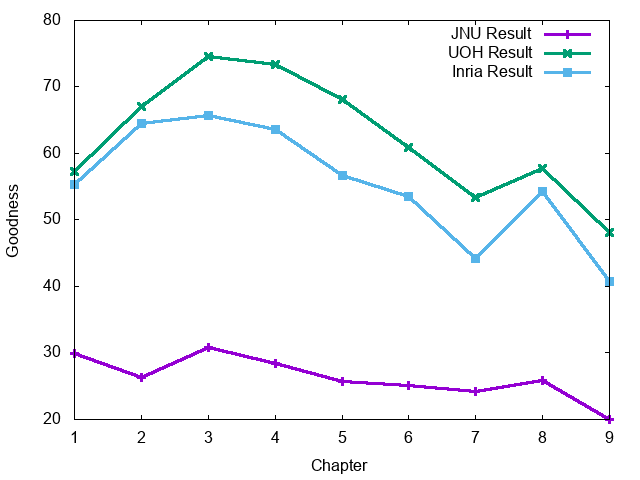
\includegraphics[scale=0.34]{images/merge.png}
	\caption{\label{gr_1}Performance of three different splitters on five different corpus for vowel type splitting.}
\end{figure}

\begin{figure}[h]
	\center
	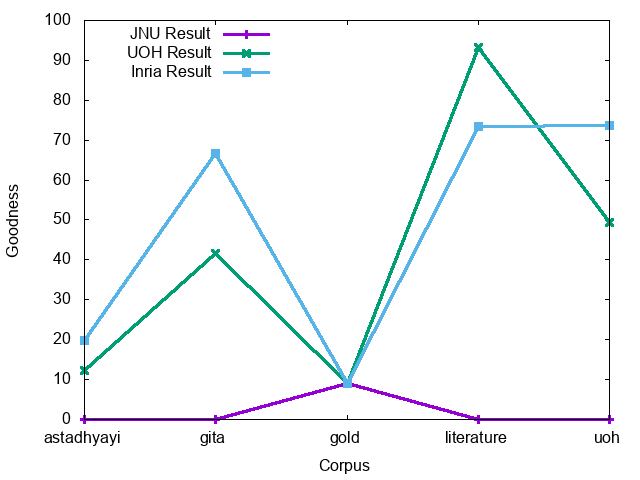
\includegraphics[scale=0.34]{images/visarga.png}
	\caption{\label{gr_2}Performance of three different splitters on five different corpus for visarga type splitting.}
\end{figure}

\begin{figure}[h]
	\center
	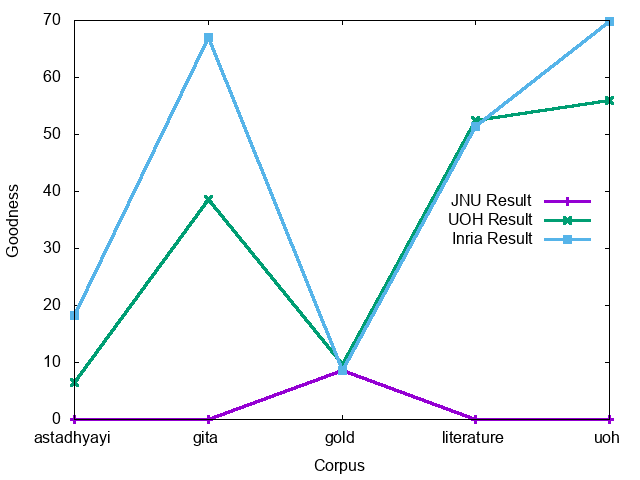
\includegraphics[scale=0.34]{images/consonant.png}
	\caption{\label{gr_3}Performance of three different splitters on five different corpus for consonant type splitting.}
\end{figure}


\section{Sandhi Merging Performance}

All of the three Sandhi merging tools allow only two words to be merged. Thus, we took first two pairs for merging and we took the resulting compound word for the next input along with its adjacent word.

\subsection{Example corpus}
We evaluated our example rule based corpus to see how many rules were implemented in each of the merging tool.
From Table~\ref{ev_ex_me}, it is clear that INRIA has the highest performance of 51\%, implying that half of the rules were not implemented by any of the tools. In UoH almost 33\% of the rules were implemented while in JNU only 21\% of the total rules were implemented.
\begin{table}[h]
	\begin{center}
		\begin{tabular}{|l|l|}
			\hline \bf Merging tool & \bf Results (282) \\ \hline
			JNU&20.9\% \\ \hline
			UoH&32.9\% \\ \hline
			INRIA&51.8\% \\ \hline
			%			\hline
		\end{tabular}
	\end{center}
	\caption{\label{ev_ex_me} Accuracy obtained using the three different merging tools in the example corpus dataset.}
\end{table}

%\subsection{Benchmark dataset}
%Results obtained on the benchmark dataset are shown in Table~\ref{ev_be_me}. Though very few rules were implemented by UoH, the performance of UoH is comparable with that of INRIA providing overwhelming above 86\% accuracy.
%\begin{table}[h]
%	\begin{center}
%		\begin{tabular}{|l  | l |}
%			\hline \bf  Merger & \bf Results (150) \\
%			\hline
%			JNU &  75 (50.0\%)\\ \hline
%			UoH &  129 (86.0\%)\\ \hline
%			INRIA & 131 (87.3\%)\\ \hline
%		\end{tabular}
%	\end{center}
%	\caption{\label{ev_be_me} Accuracy obtained using the three different merging tools in the benchmark corpus dataset.}
%\end{table}



\subsection{\textit{Bhagavad-g\={\i}t\={a}} Corpus}
Merging results for the Sandhi words of \textit{Bhagavad-g\={\i}t\={a}} corpus is shown in Table~\ref{ev_bg_me}. All the merging tools performed best for chapter three and performed badly for the chapter nine. UoH merging tool performed slightly better than the INRIA tool. Performance of UoH and INRIA tools stands at 63\% and 57\%, respectively where as JNU's performance is only 26.5\% only.

\begin{table}[h]
	\begin{center}
		\begin{tabular}{|p{1cm} | p{1cm}|p{1.2cm} | p{1.2cm} | p{1.2cm} |}
			\hline 
			\bf Chapter & \bf Words &\bf JNU & \bf UoH & \bf INRIA \\
			\hline
			
			\bf	1	&	157	&	47 (29.9\%)	&	90 (57.3\%)	&	87 (55.4\%)	\\	\hline
			\bf	2	&	270	&	71 (26.3\%)	&	181 (67.1\%)	&	174 (64.4\%)	\\	\hline
			\bf	3	&	169	&	52 (30.8\%)	&	126 (74.6\%)	&	111	(65.7\%)	\\	\hline
			\bf	4	&	165	&	47 (28.5\%)	&	121 (73.3\%)	&	105	(63.6\%)	\\	\hline
			\bf	5	&	113	&	29 (25.7\%)	&	77 (68.1\%)	&	64	(56.6\%)	\\	\hline
			\bf	6	&	187	&	47 (25.1\%)	&	114 (61.0\%)	&	100	(53.5\%)	\\	\hline
			\bf	7	&	120	&	29 (24.2\%)	&	64	(53.3\%)	&	53	(44.2\%)	\\	\hline
			\bf	8	&	116	&	30 (25.9\%)	&	67	(57.8\%)	&	63	(54.3\%)	\\	\hline
			\bf	9	&	135	&	27 (20.0\%)	&	65	(48.2\%)	&	55	(40.7\%)	\\	\hline
			\bf	Total	&	1432	&	379 (26.5\%)	&	905	(63.2\%)	&	812	(56.7\%)	\\	\hline
		\end{tabular}
	\end{center}
	\caption{\label{ev_bg_me} Accuracy obtained using the three different merging tools in the \textit{Bhagavad-g\={\i}t\={a}} corpus dataset.}
\end{table}

\subsection{UoH Corpus}
We evaluated the filtered UoH corpus using all the three merging tools and the results are shown in Table~\ref{ev_uo_me}. For UoH corpus,  UoH tool performed better than other two merging tools. 

\begin{table}[h]
	\begin{center}
		\begin{tabular}{|l|l| }
			\hline  \bf Merger & \bf Accuracy\\
			\hline
			JNU & 6517 (35.6 \%) \\ \hline
			UoH & 12895 (70.6 \%) \\ \hline
			INRIA & 12611 (68.8 \%)\\ \hline

		\end{tabular}
	\end{center}
	\caption{\label{ev_uo_me} Accuracy obtained using the three different merging tools in the UoH corpus dataset.}
\end{table}


\subsection{\textit{A\d{s}\d{t}\={a}dhy\={a}y\={\i}} Corpus}
Sandhi merging tools also performed better when the characters length is less than or equal to $20$. All three merging tools performances started decaying when the word length is increased.

\begin{table}[h]
	\begin{center}
		\begin{tabular}{|p{1cm} | p{1cm}|p{1.2cm} | p{1.2cm} | p{1.2cm} |}
			\hline  
			\bf \# letters & \bf Sandhis & \bf  JNU & \bf UoH & \bf INRIA\\
			\hline
			\bf	10	&	93	&	26 (28.0\%)	&	58 (62.4\%)	&	51 (54.8\%)	\\	\hline
			\bf	20	&	571	&	120 (21.0\%)	&	343 (60.1\%)	&	269 (47.1\%)	\\	\hline
			\bf	30	&	1512	&	250 (16.5\%)	&	763 (50.5\%)	&	634 (41.9\%)	\\	\hline
			\bf	40	&	2045	&	315 (15.4\%)	&	988 (48.3\%)	&	803 (39.3\%)	\\	\hline
			\bf	50	&	2302	&	355 (15.4\%)	&	1096 (47.6\%)	&	890 (38.7\%)	\\	\hline
			\bf	All	&	2700	&	411 (15.2\%)	&	1260 (46.7\%)	&	1016 (37.6\%)	\\	\hline

		\end{tabular}
	\end{center}
	\caption{\label{ev_as_me} Accuracy obtained using the three different merging tools in the \textit{A\d{s}\d{t}\={a}dhy\={a}y\={\i}} corpus dataset.}
\end{table}


%\subsection{Sandhi Type Based Evaluation}
%The Sandhi merging performance is evaluated on three different types of Sandhi - vowels, consonants, and visarga and the graphs are shown in Figure~\ref{gr_me_vi}, Figure~\ref{gr_me_co}, Figure~\ref{gr_me_vo}.
%JNU merger performed well in case of vowel Sandhi examples. All the merging tools performed poorly in case of consonant Sandhi. In all the three types of Sandhi, UoH merging tool performed better than the other two merging tools.
%\begin{figure}[h]
%	\center
%	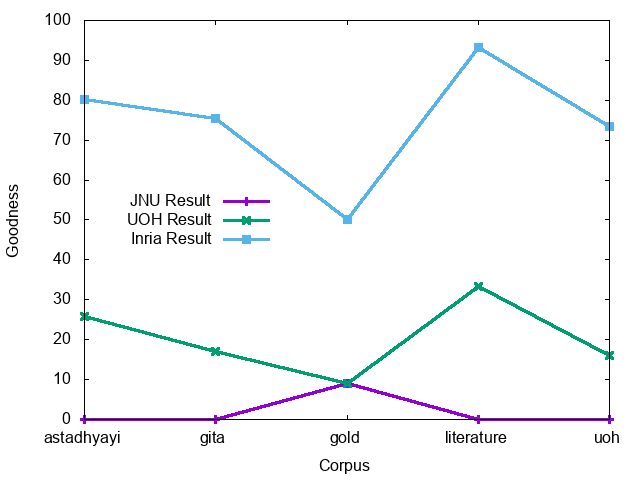
\includegraphics[scale=0.34]{images/visargamerge.png}
%	\caption{\label{gr_me_vi}Visarga Merge results}
%\end{figure}
%
%\begin{figure}[h]
%	\center
%	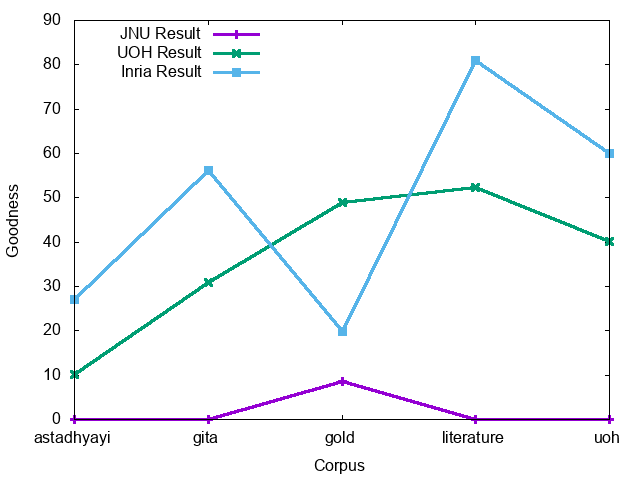
\includegraphics[scale=0.34]{images/consonantmerge.png}
%	\caption{\label{gr_me_co}Consonant Merge results}
%\end{figure}
%
%\begin{figure}[h]
%	\center
%	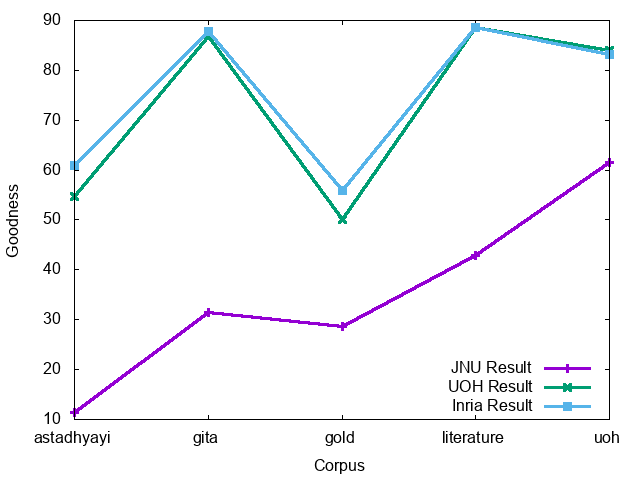
\includegraphics[scale=0.34]{images/vowelmerge.png}
%	\caption{\label{gr_me_vo}vowel merge}
%\end{figure}




\section{Discussion}
The literature based evaluation results are poor for all the three tools warranting the need for further research in this important problem. We draw attention to some of the open ended research problems and discuss them as follows:

\begin{itemize}
	\item \textbf{Rules not implemented:} Some of the less frequently used rules have not been implemented by one or more of the three splitters. For example, none of the three splitters is able to do the following split: \textit{sa yog\={\i}} $\rightarrow$ \textit{sa\d{h}} + \textit{yog\={\i}}
	
	\item \textbf{Optional rules:} There are some rules which are optional in nature and less frequently used. The following case is an example where none of the three splitters is able to detect the correct split:
	\textit{ vartanta iti} $\rightarrow$ \textit{vartante} + \textit{iti} 
	
	\item \textbf{Cascading split effect:} There are some rules in which the effect of combination of two words is not restricted to the change in sound at the extreme boundaries of the two words. For example, in
	\textit{uttara} + \textit{ayana} $\rightarrow$ \textit{uttar\={a}ya\d{n}a}, the \textit{r} of \textit{uttara} causes the change of \textit{n} of \textit{ayana} into \textit{ \d{n}}. 
	
	\item \textbf{Multiple splits:} 
	The process of Sandhi splitting involves splitting at different potential locations, and validating the splits to check which one of them is correct. If the set used for validation is not complete, even correct splits may sometimes not be validated. For example, in
	\textit{a} + \textit{chedya\d{h}} $\rightarrow$ \textit{acchedya\d{h}}, 
	the fact that none of the three splitters performed correctly is because, \textit{a} may not have been validated as a proper split.
	
	\item \textbf{Compounding effect:} The process of compounding, due to which words come together without necessarily there being a change when they merge, also creates problems. While the UoH and the INRIA tools do have the provision of decompounding along with Sandhi splitting, the JNU splitter does not have a way to do both together.
	For example, in
	\textit{lak\d{s}yasy\={a}rthatvavyavah\={a}r\={a}nurodhena} $\rightarrow$  \textit{lak\d{s}yasya} + \textit{arthatvavyavah\={a}ra} + \textit{anurodhena} 
	the second split is not validated without decompounding, and thus even though, only vowel sandhis are involved, the JNU splitter is not able to correctly split the word.  
\end{itemize}




\section{Conclusion}
In this research, we discussed different tools that implement Sanskrit Sandhi merging and splitting mechanisms. We created five manually curated public datasets to benchmarking both Sandhi merging and splitting. Also, we curated ambiguous existing corpus to get reasonably accurate Sandhi corpus. 
Further, we benchmarked three public tools for Sandhi splitting and merging on our dataset - INRIA, JNU, and UoH. From our experiments, it is evident that in case of Sandhi splitting INRIA performed better whereas JNU performed very poorly. In case of Sandhi merging, UoH and INRIA performed almost equivalently while JNU again performed poorly in case of merging also. 
For Sandhi merging the number of rules that were implemented in all the three tools is only 50\%, which opens the door for implementation of other rules which were missing. We strongly hope that the research community could make the best use of the benchmark dataset to improve the performance of Sanskrit language understanding.

\newpage
{
	\bibliographystyle{eacl2017}
	\bibliography{eacl2017}
}

\end{document}
